\section{WSNET}

\subsection{Code availability and reproduction of the results}

Although the code for WSNET \cite{Oota_2023_WACV} is stated to be publicly available, a closer inspection of the linked GitHub repository shows, that this is only partially the case. A lack of documentations makes it hard to make use of the code, especially since the code seems to contain some errors.

In the scope of this project, the code was used to create runable models again. Unfortunately, the classes of the wounds are not available, which makes it impossible to perform pre-training as it was described in the original paper \cite{Oota_2023_WACV}. In total there are eight models available: A local model and a combined global-local model for each of the segmentation models Unet, PSPNet, FPN, and Linknet. The Python library used for the segmentation models is \texttt{segmentation\_models} \cite{SegmentationModels}. The implementation processed showed some differences to the described model architecture. In particular, it was claimed that the wound images were split up in parts of 48\,px times 48\,px. However, three of the four models, all beside PSPNet, only allow input sizes that are divisable by 32 and the GitHub showed a size of 64\,px was used. Another difference between available code and the paper is, that it is claimed that augmentation is not performed on the test images which is not the case in the available code.

Information about the size of training, validation and test set is not given in the paper or code. In the scope of this project, a split of 70\,\% training, 15\,\% validation and 15\,\% test data is used.

\begin{itemize}
	\item train + validation set were just first x\,\% of dataset, not shuffled as one would normally do it
\end{itemize}

Because the data training for the wound-specific pre-training is not available, the results can only be compared for imagenet pre-training.


\begin{itemize}
	\item problem with imagenet pretraining: input size for patches is not available, instead the default size of 224 is used, which might impact results negatively
\end{itemize}


\subsection{Comparison of the achieved performance}

\begin{table}[htb!]
	\centering
	\begin{tabular}{l||c | c | c | c | c | c | c | c|}
	& \multicolumn{2}{|c|}{Unet} & \multicolumn{2}{|c|}{Linknet} & \multicolumn{2}{|c|}{PSPNet} & \multicolumn{2}{|c|}{FPN} \\
	\hline
	& IoU & Dice & IoU & Dice & IoU & Dice & IoU & Dice \\
	\hline\hline
	\textbf{Local model} & 0.359 & 0.523 & 0.398 & 0.564 & 0.373 & 0.538 & 0.408 & 0.574 \\	
	\textbf{Global model} & 0.504 & 0.668 & 0.631 & 0.772 & 0.458 & 0.627 & 0.632 & 0.772 \\
	\textbf{Global-Local model} & 0.495 & 0.658 & 0.618 & 0.763 & 0.476 & 0.642 & 0.612 & 0.758\\
	\end{tabular}
	\caption{IoUe-Scores and Dice Coefficients for the four different models with each Global-Local, Global and Local architecture. The backbone used is mobilenet.}
\end{table}

\begin{figure}[htb!]
	\centering
	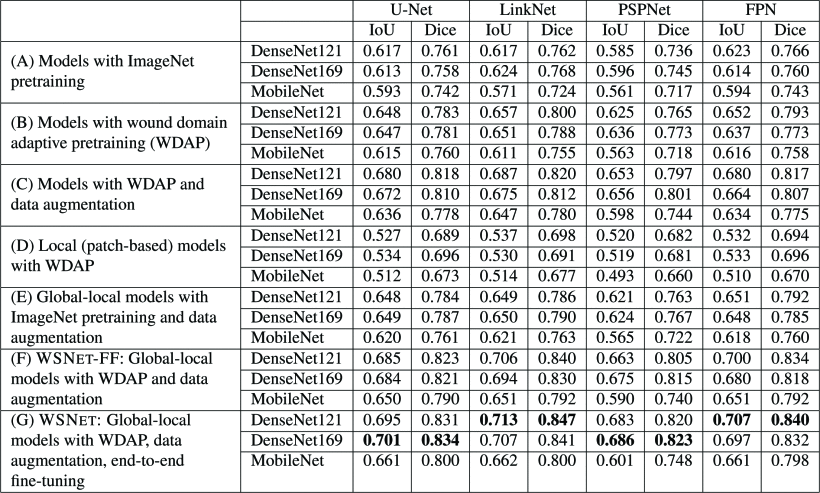
\includegraphics[width=\textwidth]{fig/wsnet-results.png}
	\caption{Results reported by \citeauthor{Oota_2023_WACV} \cite{Oota_2023_WACV}.}
\end{figure}

\begin{itemize}
	\item results are comparable with results reported in paper, slightly lower scores
	\item e.g. Unet IoU score 0.495 with my code, 0.620 in paper (dice score 0.761 vs 0.658)
	\item others are closer (linknet 0.618 from me vs 0.621 in paper, dice 0.763 in paper and for me)
	\item maybe differences in training size
	\item most important thing: the global-local model does not improve about global model
	\item TODO: explain here or later??
	\item the results reported by \citeauthor{Oota_2023_WACV} are shown in figure
\end{itemize}
